% Source of report_extended.pdf. Build in this folder with two runs of
%   xelatex -jobname=report_extended main.tex
% (fonts: TeX Gyre Termes/Heros, STIX Two Math, Noto Serif CJK SC) and copy report_extended.pdf to ../
\documentclass[a4paper,11pt]{article}
\usepackage{fontspec}
\setmainfont{TeX Gyre Termes}
\setsansfont{TeX Gyre Heros}
\newfontfamily\cjkfont{Noto Serif CJK SC}
\usepackage{amsmath}
\usepackage{unicode-math}
\setmathfont{STIXTwoMath-Regular.otf}
\usepackage[a4paper,top=2.5cm,bottom=2.4cm,left=2.6cm,right=2.6cm]{geometry}
\usepackage{graphicx,booktabs,array,threeparttable,pdfpages,fancyhdr,xurl}
\usepackage[font=small,labelsep=period,skip=4pt]{caption}
\usepackage[hidelinks,bookmarksnumbered=true,bookmarksopen=true]{hyperref}
\usepackage{titlesec}
\renewcommand{\floatpagefraction}{0.8}\renewcommand{\topfraction}{0.88}\renewcommand{\bottomfraction}{0.7}\renewcommand{\textfraction}{0.1}
\usepackage{etoolbox}\AtBeginEnvironment{thebibliography}{\small\linespread{1.05}\selectfont\setlength{\itemsep}{1pt}\setlength{\parskip}{0pt}}
\setlength{\emergencystretch}{3em}
\linespread{1.15}
\setlength{\parskip}{0.25em}
\titleformat{\section}{\large\bfseries}{E\arabic{section}}{0.8em}{}
\titleformat{\subsection}{\normalsize\bfseries}{E\arabic{section}.\arabic{subsection}}{0.6em}{}
\renewcommand{\thesection}{E\arabic{section}}
\renewcommand{\thefigure}{E\arabic{figure}}
\renewcommand{\thetable}{E\arabic{table}}
\renewcommand{\theequation}{E\arabic{equation}}
\setlength{\headheight}{15pt}\pagestyle{fancy}\fancyhf{}\renewcommand{\headrulewidth}{0.4pt}
\newcommand{\hd}[1]{\begin{tabular}[b]{@{}c@{}}#1\end{tabular}}
\newcommand{\exthead}[1]{\fancyhead[L]{\small #1}\fancyhead[R]{\small Part II\quad Post-competition extensions}\fancyfoot[C]{\small E-\thepage}}

\graphicspath{{../../figures/extension/}}
\hypersetup{pdftitle={Noise-adaptive quantum compiler -- extended edition}}
\begin{document}
\thispagestyle{empty}
\begin{center}
{\Large\bfseries Noise-Adaptive Quantum Compiler\\[0.2em] for a Dual-Track NISQ Mapping Challenge}\\[0.7em]
{\large Extended edition --- note}
\end{center}
\vspace{0.8em}

This file has two parts. Part I is the submission report of the 2026 noise-adaptive quantum compilation challenge (9 pages), reproduced exactly as submitted. Part II, starting on page E-1, contains post-competition extensions written in November 2026.

The compiler maps circuits onto noisy hardware snapshots with noise-weighted layout and look-ahead routing, structure-specific synthesis and a proof-carrying relative-phase Toffoli rewrite, and selects among candidate compilations with a reliability proxy. On the public evaluation it scores 0.833 against 0.663 for the organisers' baseline. Part II tests two things the public set cannot show. E1 builds two new suites in the challenge format, unseen circuit sizes from the organisers' own generator and independently written QASMBench circuits, and finds that the advantage over the baseline carries over ($+0.108$ and $+0.065$ in success probability, with about 35\,\% fewer two-qubit gates); it also exposes a failure mode, compile time on the largest circuits, and evaluates a deadline guard that removes it. E2 scores every candidate compilation exactly with a density-matrix simulation under the evaluator's noise model and shows that candidate selection is saturated: the best candidate in each pool beats the submitted choice by only 0.0004 on average, so further gains must come from candidate generation.

Every number in Part II can be reproduced with the scripts in the \texttt{extension/} folder of the code repository; result files are in \texttt{results/extension/}.

\clearpage
\pdfbookmark[0]{Part I\quad Submission report (as submitted)}{part1}
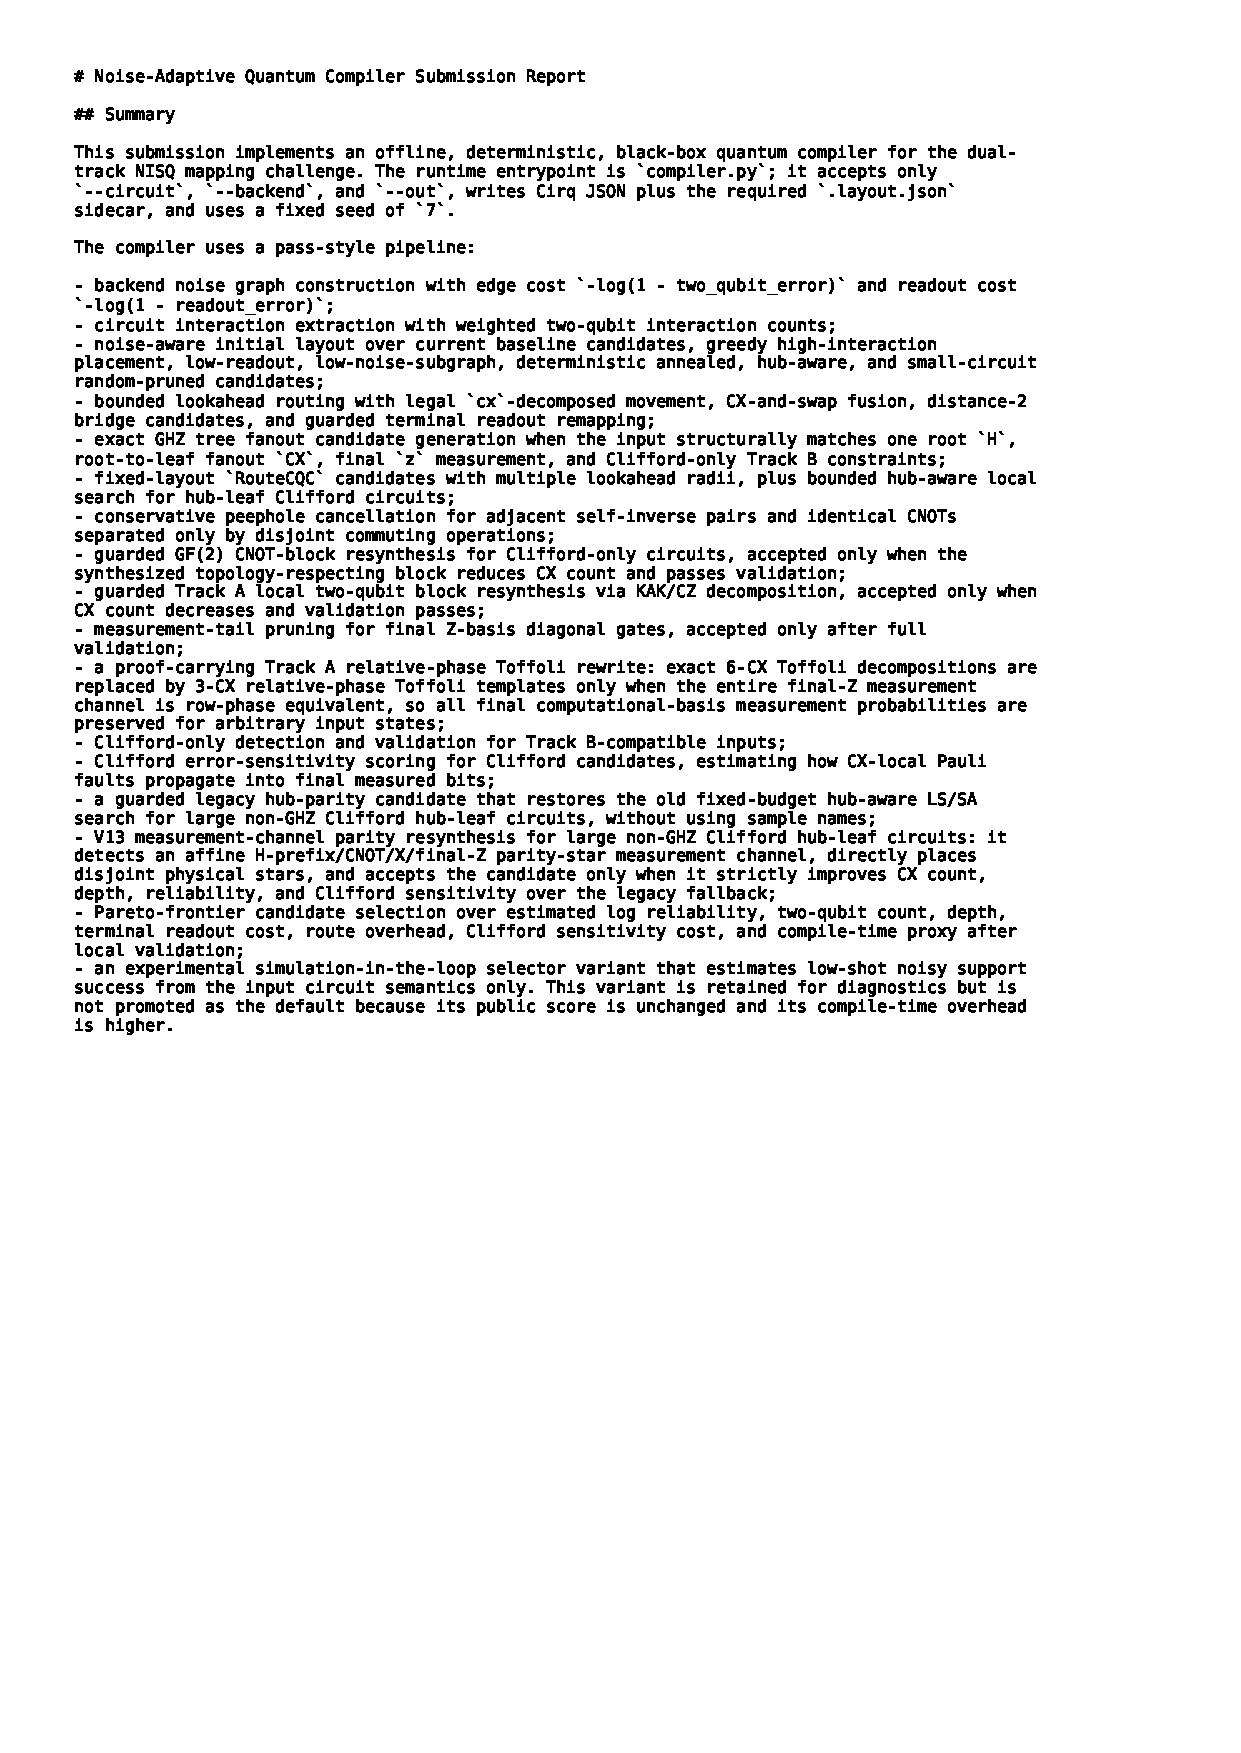
\includepdf[pages=-]{../report.pdf}
\pdfbookmark[0]{Part II\quad Post-competition extensions}{part2}
\setcounter{page}{1}
\exthead{Noise-adaptive quantum compiler}
\begin{center}{\Large\bfseries Part II\quad Post-competition extensions}\end{center}

The challenge scores a black-box compiler by the noisy success probability of each compiled circuit: Track A consists of general NISQ circuits simulated with Cirq, Track B of large Clifford circuits simulated with Stim\cite{stim}, and the final score is $0.75A+0.25B$. Every output must pass the validator, an equivalence check and a noiseless semantic check. The submission combines noise-adaptive layout and routing in the spirit of Murali et al.\cite{murali} with structure-specific synthesis and a proof-carrying rewrite of exact Toffoli decompositions into relative-phase Toffoli gates\cite{maslov}, and it selects among candidate compilations with a reliability proxy. On the public evaluation (seven seeds) the submission scores 0.894 on Track A and 0.650 on Track B, a final score of 0.833 against 0.663 for the organisers' baseline, with no invalid outputs. The public Track A set, however, contains only eight circuits of six or seven qubits, and the compiler's design decisions were tuned against it. Two questions therefore remain open. E1 asks whether the advantage generalises to circuits the compiler was not developed on. E2 asks how much of the remaining gap to the best achievable compilation is due to the selection step, which chooses one candidate from a pool of valid compilations, and how much is due to the pool itself.

\section{Generalisation beyond the eight public Track A circuits}

\subsection{Design}
Two suites were built in the challenge format. Suite S1 contains every Track A family of the organisers' generator at 5, 8 and 11 program qubits with two generator seeds, which gives 46 circuits on the medium 16-qubit backend (the adder family has no 5-qubit instance). Suite S2 contains the 11 of 25 small QASMBench circuits\cite{qasmbench} that parse into the challenge's gate set, have 2--11 qubits and either a deterministic output or an output support of at most $\min(2^{n-2},16)$ bitstrings: two ripple-carry adders\cite{cuccaro}, Toffoli and Fredkin gates, a hidden-shift instance, Grover search, learning parity with noise, a quantum error-correction encoder, a satisfiability instance, a cat state and an iSWAP circuit. Their measurements are stripped and every qubit is re-measured, so that each circuit has a well-defined set of accepted output bitstrings. Both suites are scored with the organisers' evaluator against their RouteCQC baseline at seeds 7 and 11 with 256 shots, under the same validity checks as the challenge.

\subsection{Results}

\begin{table}[htbp]\centering\small\setlength{\tabcolsep}{4.5pt}
\caption{Mean success probability of the submission and the organisers' RouteCQC baseline on the two generalisation suites (seeds 7 and 11, 256 shots, 60-s compile limit). Circuit--seed pairs count as better or worse when the difference exceeds 0.02; CX is the mean number of two-qubit gates after compilation.}\label{tab:lxb-e1}
\begin{tabular}{lccccc}\toprule
Suite & Submission & Baseline & Gap & Pairs better / worse & CX, subm. / baseline\\\midrule
S1 unseen sizes ($46\times2$) & 0.831 & 0.723 & $+0.108$ & 87 / 3 & 9.6 / 14.8\\
S2 QASMBench ($11\times2$) & 0.818 & 0.753 & $+0.065$ & 18 / 1 & 18.6 / 28.9\\\bottomrule
\end{tabular}
\end{table}

\begin{table}[htbp]\centering\small\setlength{\tabcolsep}{4pt}
\caption{Success probability by family (S1) and by circuit (S2), mean over both seeds. The S2 adder\_n10 value of the submission includes one compile-time failure scored as zero.}\label{tab:lxb-e1b}
\begin{tabular}{lccc@{\hspace{2.2em}}lccc}\toprule
S1 family & Subm. & Baseline & Gap & S2 circuit & Subm. & Baseline & Gap\\\midrule
adder & 0.750 & 0.550 & $+0.200$ & adder\_n4 & 0.889 & 0.812 & $+0.076$\\
Bernstein--Vazirani & 0.871 & 0.829 & $+0.042$ & adder\_n10 & 0.121 & 0.127 & $-0.006$\\
Fredkin & 0.875 & 0.759 & $+0.116$ & cat\_state\_n4 & 0.947 & 0.930 & $+0.018$\\
hidden shift & 0.822 & 0.725 & $+0.097$ & fredkin\_n3 & 0.920 & 0.793 & $+0.127$\\
OR & 0.896 & 0.791 & $+0.105$ & grover\_n2 & 0.961 & 0.930 & $+0.031$\\
Peres & 0.885 & 0.754 & $+0.131$ & hs4\_n4 & 0.936 & 0.898 & $+0.037$\\
structured random & 0.637 & 0.521 & $+0.116$ & iswap\_n2 & 0.975 & 0.953 & $+0.021$\\
Toffoli & 0.882 & 0.794 & $+0.089$ & lpn\_n5 & 0.945 & 0.893 & $+0.053$\\
 & & & & qec\_en\_n5 & 0.855 & 0.834 & $+0.021$\\
 & & & & sat\_n7 & 0.516 & 0.268 & $+0.248$\\
 & & & & toffoli\_n3 & 0.932 & 0.848 & $+0.084$\\\bottomrule
\end{tabular}
\end{table}

\begin{figure}[htbp]\centering
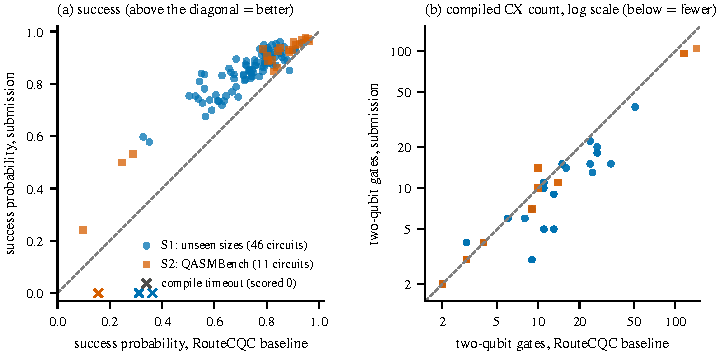
\includegraphics[width=0.8\textwidth]{figE1_generalisation.pdf}
\caption{Submission against the RouteCQC baseline on the two generalisation suites, per circuit and seed. (a) Success probability (above the diagonal: the submission is better); crosses mark compile-time failures scored as zero. (b) Two-qubit gate count after compilation, logarithmic scale (below the diagonal: the submission uses fewer gates).}\label{fig:lxb-e1}
\end{figure}

The advantage carries over to new sizes and to independently written circuits (Table~\ref{tab:lxb-e1}, Figure~\ref{fig:lxb-e1}). On S1 the submission is better in 87 of 92 circuit--seed pairs and worse in 3, and on S2 better in 18 of 22 and worse in one. The mechanism is visible in the gate counts: the submission uses about 35\,\% fewer two-qubit gates on both suites, and two-qubit gates carry the largest error rates of the hardware snapshots. In line with this mechanism, the gain tends to be larger where there is more two-qubit work to remove (Table~\ref{tab:lxb-e1b}). It is largest for the adders of S1 ($+0.200$) and for the seven-qubit satisfiability circuit of S2 ($+0.248$), whose input already contains 80 CX gates, and small ($+0.018$ to $+0.031$) for the cat-state, iSWAP and two-qubit Grover circuits, which contain only two or three CX gates and leave little to optimise. The relation is not strict: the error-correction encoder, with ten CX gates, gains similarly little ($+0.021$).

\subsection{A failure mode: compile time}

The only S2 circuit on which the submission loses is the ten-qubit QASMBench adder, whose input has 81 CX gates, and the loss is not a matter of compilation quality. With seed 7 the compiler needed 49.6 s and produced 104 CX gates against 144 for the baseline; with seed 11 it exceeded the 60-s limit of the evaluation and the sample was scored as invalid. The 11-qubit structured-random instance of S1 timed out under both seeds. Under the official 30-s limit the adder fails as well. The compiler therefore has no protection against its own search time on the largest circuits, which in the challenge would turn a moderate score into zero. A deadline guard addresses this: it runs the submitted compiler with an internal budget of 24 s and emits the RouteCQC baseline if the budget is exceeded, so that a slow compilation degrades to the baseline score instead of an invalid sample.

\begin{table}[htbp]\centering\small
\caption{Effect of the deadline guard under the official 30-s compile limit (seed 7).}\label{tab:lxb-e1c}
\begin{tabular}{lccc}\toprule
Suite & Submission & Guarded submission & Invalid samples (submission $\to$ guarded)\\\midrule
S1 unseen sizes & 0.829 & 0.836 & $1\to0$\\
S2 QASMBench & 0.801 & 0.810 & $1\to0$\\\bottomrule
\end{tabular}
\end{table}

With the guard, both suites are free of invalid samples and their scores rise to 0.836 and 0.810 (Table~\ref{tab:lxb-e1c}). The guard costs nothing on circuits that compile in time, because it returns the submitted compiler's output unchanged.

\section{How much does candidate selection leave on the table?}

\subsection{Design}
The compiler builds a pool of valid compilations for each circuit and selects one in two steps. A reliability proxy, the sum of $\log(1-\varepsilon)$ over all gates and readouts with Pareto guards on two-qubit count, depth, readout cost and Clifford fault sensitivity, ranks the pool; the proxy's choice and its top eight candidates are then re-scored by a 512-shot noisy simulation with common random numbers, and the choice is replaced only if another candidate wins by more than 0.006. At the success levels involved a 512-shot estimate has a standard error of about 0.015--0.02, so the second step can keep a worse candidate or select a lucky one. E2 removes all sampling noise. Every candidate in every pool is scored by its exact expected success: the density matrix of the compiled circuit is computed under the evaluator's own noise model, with depolarising channels after every gate and bit-flip readout errors as in the organisers' Cirq runner, and its probability mass on the accepted bitstrings is summed. Selection rules are then compared on identical pools, and the score of a rule is the exact success of the candidate it selects.

Of the 65 circuits (8 public, 46 from S1 and 11 from S2), 57 were scored exactly: 8 public, 39 from S1 and 10 from S2, with 1\,520 candidates in total. In the other eight, namely the four hidden-shift instances of S1, both 11-qubit structured-random instances, one 11-qubit Bernstein--Vazirani instance and the ten-qubit QASMBench adder, dense density-matrix simulation of at least one candidate took more than 60 s, and such circuits are excluded whole rather than scored on part of their pool.

\subsection{Results}

\begin{table}[htbp]\centering\small
\caption{Selection rules compared by the exact expected success of the selected candidate (57 circuits).}\label{tab:lxb-e2}
\begin{tabular}{lcc}\toprule
Selection rule & Mean exact success & Circuits below the best in the pool\\\midrule
Proxy with Pareto guards & 0.8752 & 7\\
Raw proxy, top candidate & 0.8756 & 4\\
Submitted (proxy + 512-shot re-scoring) & 0.8754 & 5\\
Exact evaluation of the proxy's top 8 & 0.8758 & 1 (by $2\times10^{-6}$)\\
Best candidate in the pool & 0.8758 & ---\\\bottomrule
\end{tabular}
\end{table}

\begin{figure}[htbp]\centering
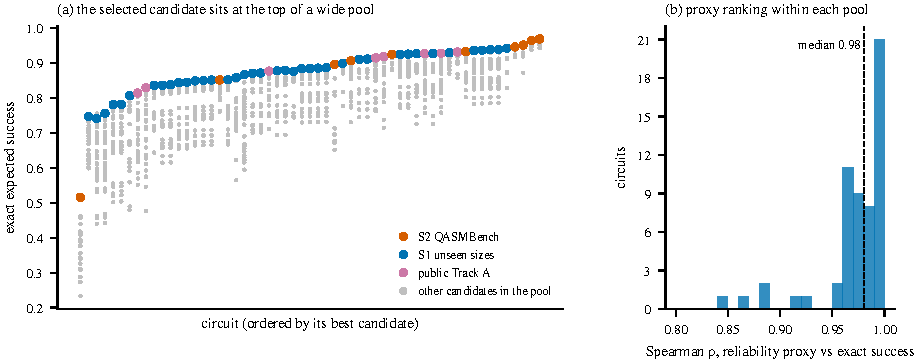
\includegraphics[width=0.9\textwidth]{figE2_selection_headroom.pdf}
\caption{(a) Exact expected success of every candidate in each pool (grey) and of the candidate selected by the submitted rule (coloured by suite). (b) Per-circuit rank correlation between the reliability proxy and exact success.}\label{fig:lxb-e2}
\end{figure}

Selection is saturated (Table~\ref{tab:lxb-e2}). The best candidate in the pool beats the submitted choice by only 0.0004 on average, and by at most 0.014, in one 11-qubit adder. Exact scoring of the eight candidates that the submission already re-scores would recover all of this headroom except $2\times10^{-6}$ in a single circuit; since the shot sampler draws from the same density matrix, this would cost about as much as one 512-shot run, but it would gain less than a thousandth in success probability.

The saturation is not a consequence of uniform pools. The pools are wide: the best and the worst candidate differ by 0.18 on average and the best and the median candidate by 0.047, so a poor selection rule would lose a great deal. The reliability proxy nevertheless ranks the pools almost perfectly (Figure~\ref{fig:lxb-e2}). The median per-circuit Spearman correlation between proxy and exact success is 0.98, the minimum is 0.84, and the proxy's top candidate is the exact best in 93\,\% of circuits. This agrees with the structure of the noise model: with independent depolarising and readout channels and a small set of accepted outputs, the logarithm of the success probability is approximately additive in the per-operation error rates, which is what the proxy sums.

The additional machinery does not pay. The 512-shot re-scoring changed the guarded proxy's choice in four circuits, for the better in three (by up to $+0.010$) and for the worse in one ($-0.014$), which averages $+0.0002$ over the 57 circuits. The raw proxy's top candidate is as good as the full pipeline (0.8756 against 0.8754), and two of the four circuits in which it misses the best candidate miss it by less than $2\times10^{-5}$. The Pareto guards themselves cost 0.0004 on this set (0.8752 against 0.8756). Further improvement must therefore come from candidate generation, that is, from better layouts, routing and synthesis, and not from selection.

\subsection{Conclusions and limits}

The compiler's advantage over the organisers' baseline is not an artefact of the eight public circuits: it holds on 46 generated circuits of unseen sizes and on 11 external circuits, and its source, the removal of about a third of the two-qubit gates, is the same throughout. Its weakness is compile time on the largest circuits, which a deadline guard turns from an invalid sample into a baseline-level result. The selection step is already close to optimal on every circuit that could be scored exactly. Three limits apply. The suites are small, with two seeds per circuit and the deadline guard evaluated on seed 7 only. S1 comes from the organisers' own generator, so it tests new sizes rather than new structures, while S2 tests new structures but at small scale. The exact analysis covers circuits whose candidates can be simulated densely within 60 s, which excludes the largest circuits, where shot noise and proxy error are most likely to matter; for those circuits the size of the selection headroom remains unmeasured.

\begin{thebibliography}{9}
\bibitem{stim} C. Gidney. Stim: a fast stabilizer circuit simulator. \emph{Quantum}, 5: 497, 2021. doi:10.22331/q-2021-07-06-497.
\bibitem{qasmbench} A. Li, S. Stein, S. Krishnamoorthy, J. Ang. QASMBench: a low-level quantum benchmark suite for NISQ evaluation and simulation. \emph{ACM Transactions on Quantum Computing}, 4(2): 10, 2023. doi:10.1145/3550488.
\bibitem{cuccaro} S. A. Cuccaro, T. G. Draper, S. A. Kutin, D. P. Moulton. A new quantum ripple-carry addition circuit. arXiv:quant-ph/0410184, 2004.
\bibitem{murali} P. Murali, J. M. Baker, A. Javadi-Abhari, F. T. Chong, M. Martonosi. Noise-adaptive compiler mappings for noisy intermediate-scale quantum computers. In \emph{Proceedings of ASPLOS 2019}, 1015--1029. doi:10.1145/3297858.3304075.
\bibitem{maslov} D. Maslov. Advantages of using relative-phase Toffoli gates with an application to multiple control Toffoli optimization. \emph{Physical Review A}, 93: 022311, 2016. doi:10.1103/PhysRevA.93.022311.
\end{thebibliography}
\end{document}
